\documentclass{standalone}
\usepackage{tikz}
\usetikzlibrary{shapes.geometric, arrows.meta}
\usetikzlibrary{arrows}

\definecolor{darkblue}{HTML}{00639a}
\definecolor{darkred}{HTML}{e41a1c}
\definecolor{darkgreen}{HTML}{4daf4a}
\definecolor{darkpink}{HTML}{ea147e}

\definecolor{lightpink}{HTML}{ffccd7}
\definecolor{lightblue}{HTML}{4ccdff}



\begin{document}
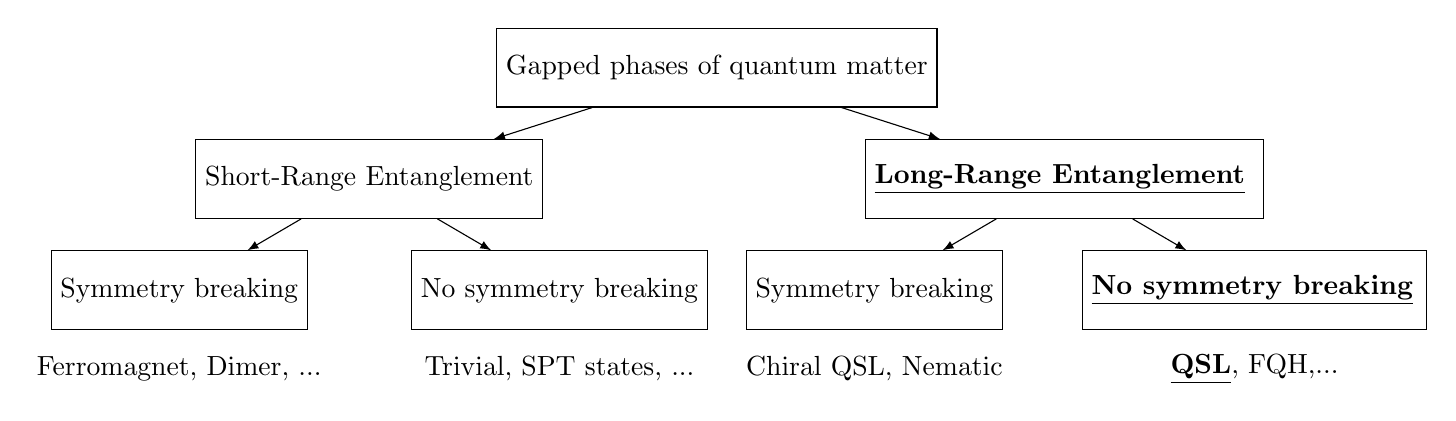
\begin{tikzpicture}[>=latex,node distance=2cm,  node1/.style={rectangle, draw, align=center, minimum width=2cm, minimum height=1cm}]

% Central node
\node[node1] (central) {Gapped phases of quantum matter};

% First bifurcation
\node[node1] (left1) [below left of=central, xshift=-3cm] {Short-Range Entanglement};
\node[node1] (right1) [below right of=central, xshift=3cm] { \textbf{\underline{Long-Range Entanglement}} };

% Second bifurcation
\node[node1] (left2a) [below left of=left1, xshift=-1cm] {Symmetry breaking};
\node[node1] (left2b) [below right of=left1, xshift=1cm] {No symmetry breaking};
\node[node1] (right2a) [below left of=right1, xshift=-1cm] {Symmetry breaking};
\node[node1] (right2b) [below right of=right1, xshift=1cm] {\textbf{\underline{No symmetry breaking}}\! };

% Draw edges
\draw[->] (central) -- (left1);
\draw[->] (central) -- (right1);
\draw[->] (left1) -- (left2a);
\draw[->] (left1) -- (left2b);
\draw[->] (right1) -- (right2a);
\draw[->] (right1) -- (right2b);



% third line
\node (left3a) [below of=left2a, yshift=1cm] {Ferromagnet,   Dimer,  ...};
\node (left3b) [below  of=left2b, yshift=1cm] {Trivial,  SPT states,  ...};
\node (right3a) [below  of=right2a, yshift=1cm] {Chiral QSL,  Nematic };
\node (right3b) [below  of=right2b, yshift=1cm] {\textbf{\underline{QSL}}, FQH,...};



\end{tikzpicture}
\end{document}
